In order to optimize the continuous time models we choose to use reinforcement learning methods, the following section covers the Markov Decision Process formalism and gives an introduction to the main ideas behind Proximal Policy Optimization (PPO) \cite{schulman2017ppo}, the algorithm that we will use to train our model. \\% This formulation has several advantages, first it enables the training of the model to happen without any exterior intervention or training data, and secondly it will enable us to 

\subsection{Markov Decision Processes}

\begin{figure}[h!]
    \centering
    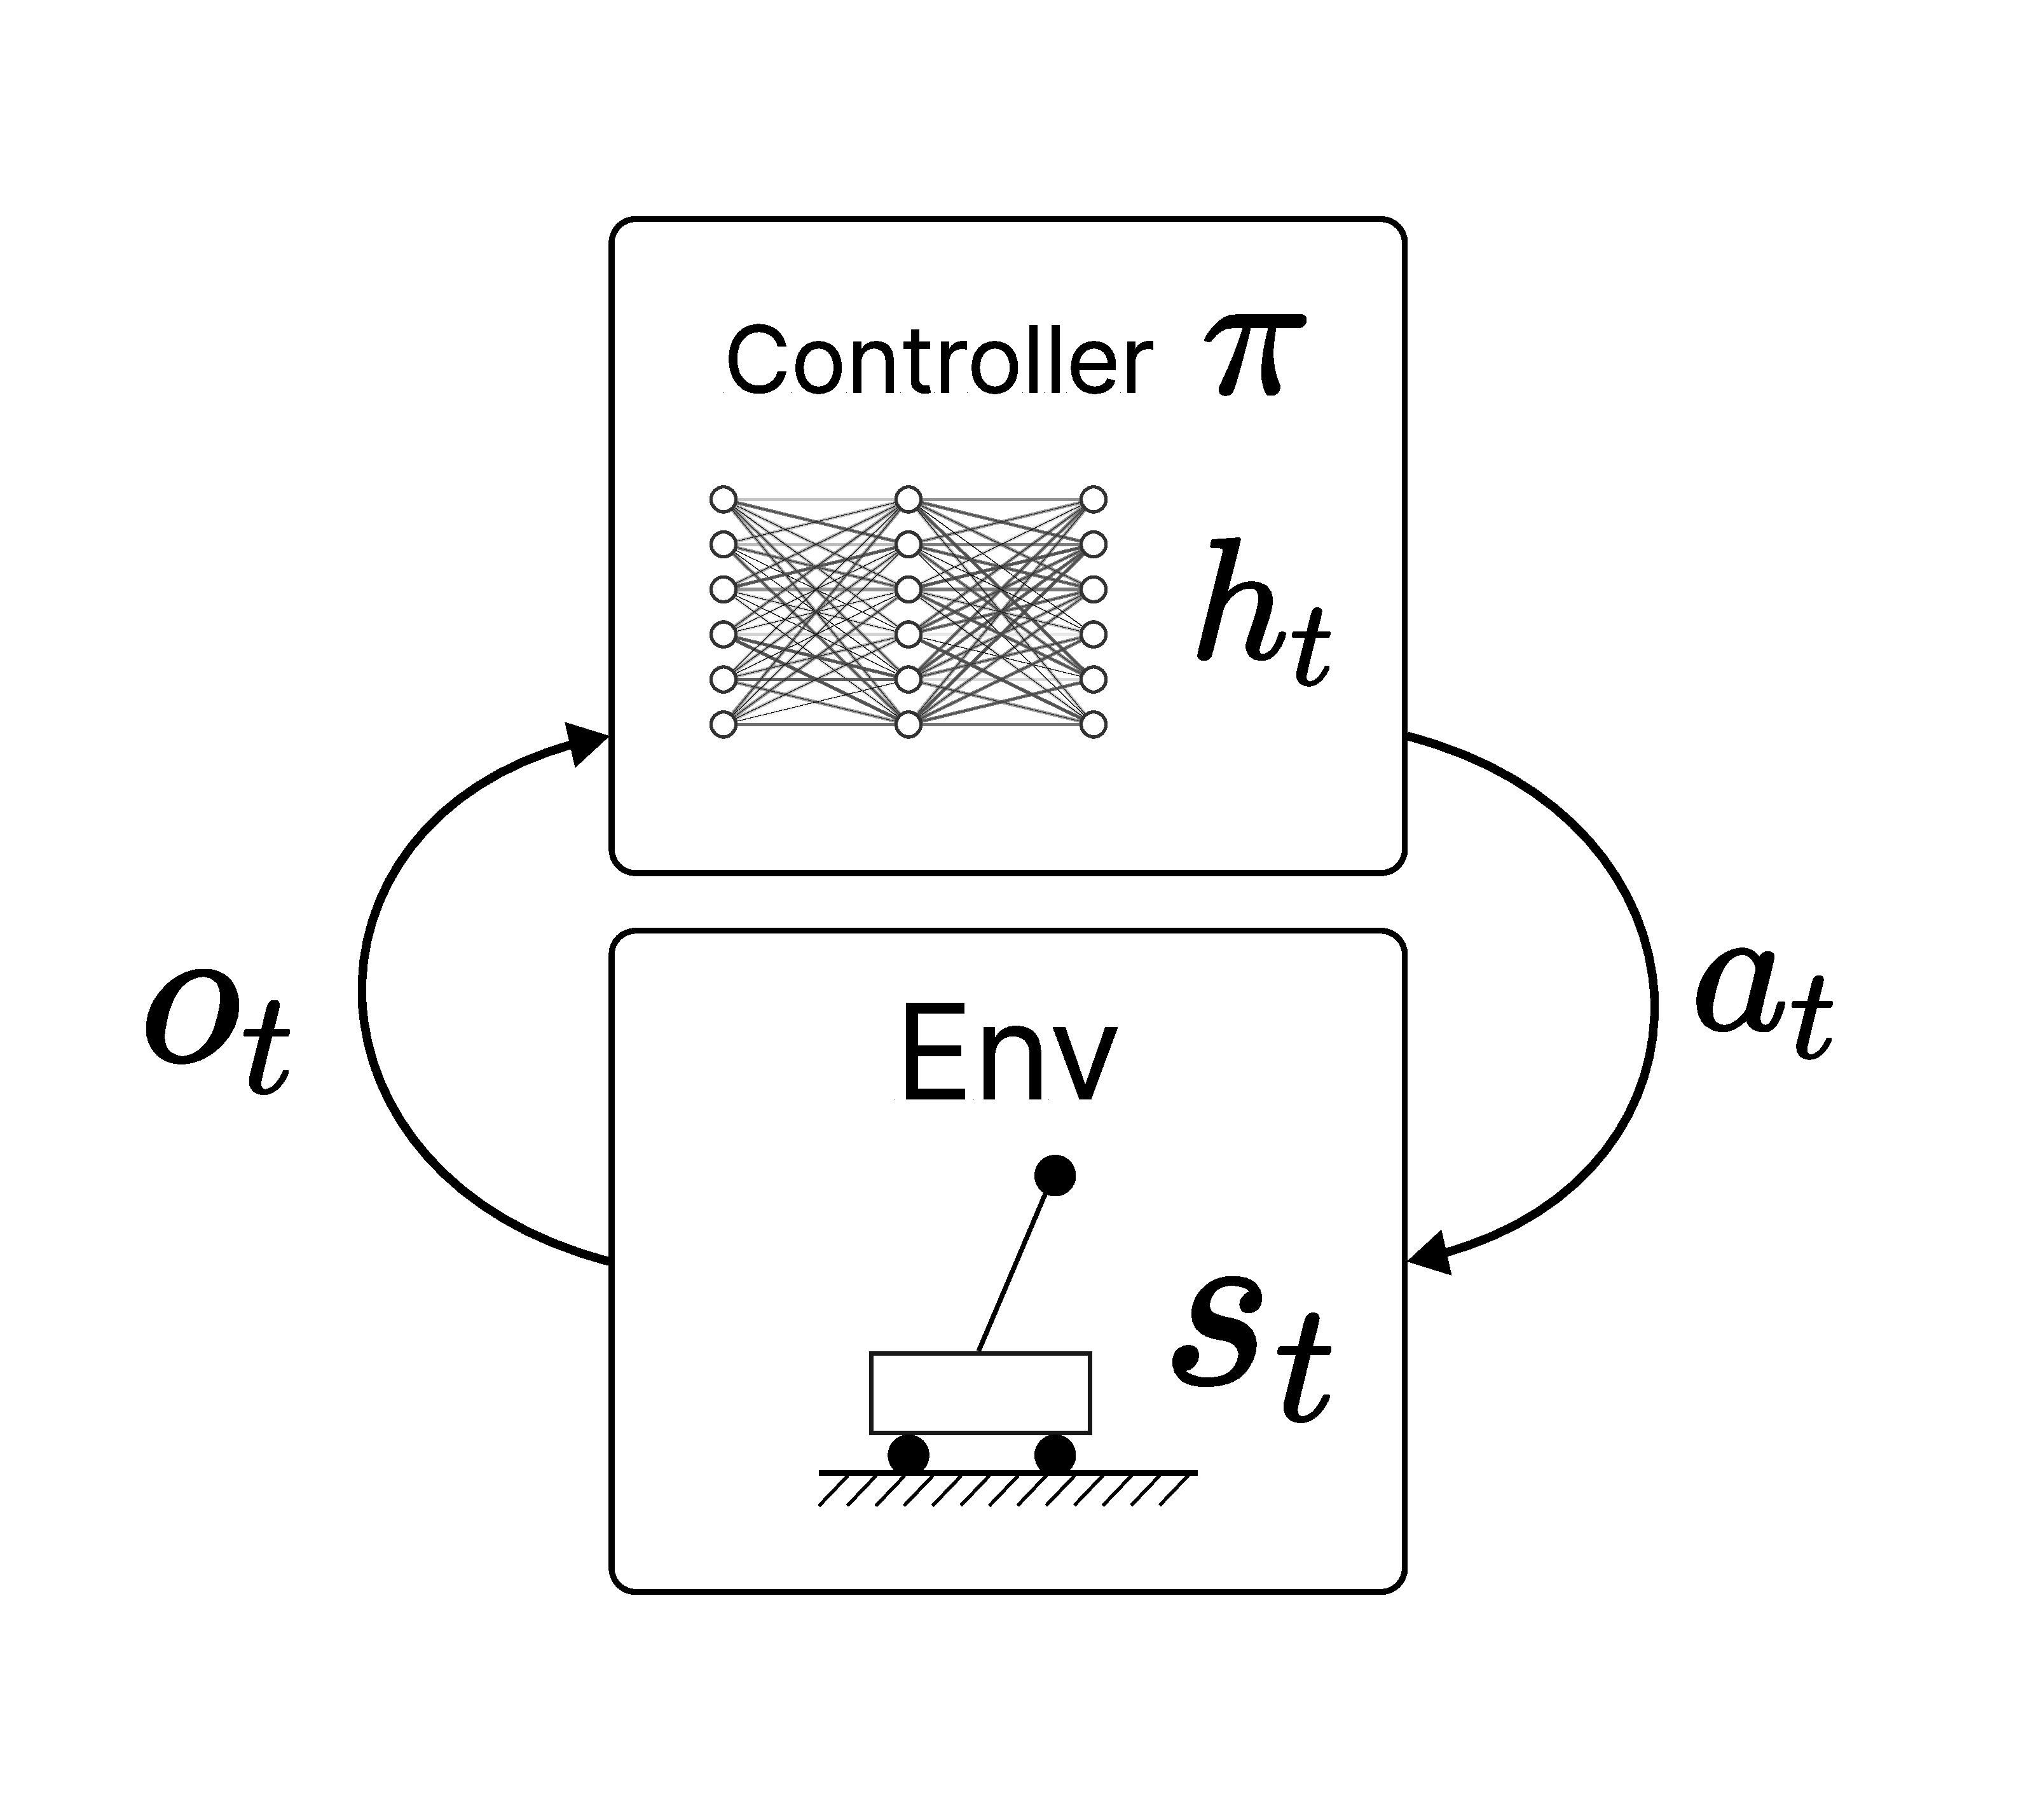
\includegraphics[width=0.45\textwidth]{figures/system.pdf}
    \caption{A visual representation of the different components required to define an RL problem. An environment, which keeps state and defines the transition probability function, and a policy function (which may have a hidden state $h$) which takes observations $o_t$ of $s_t$ as inputs and returns actions $a_t$ as outputs.}
\end{figure}

Formulating our control problem as a reinforcement learning problem requires us to write out a control task as a partially observable Markov decision process (POMDP). We define a POMDP through:
\begin{enumerate}
    \item a (partially observable) state space $\mathcal{S}$ with states $s_t\in \mathbb{R}^n$,
    \item an observation space $\mathcal{O}$ with states $o_t\in \mathbb{R}^m$, where observations $o_t$ give some information about the true states $s_t$,
    \item an action space $\mathcal{A}$ with action $a_t \in \mathcal{A}\subseteq\mathbb{R}^d$, which gives the possible actions that the agent can take in a given state,
    \item an unknown transition probability function $P(s_{t+1}|s_{t},a_{t})$, which gives the probability that the system transitions to state $s_{t+1}$ if it is in state $s_{t}$ and action $a_t$ is taken,
    \item a reward function $R:(s_{t+1},s_t,a_t) \rightarrow \mathbb{R}$.
\end{enumerate}

\begin{figure}[h!]
    \centering
    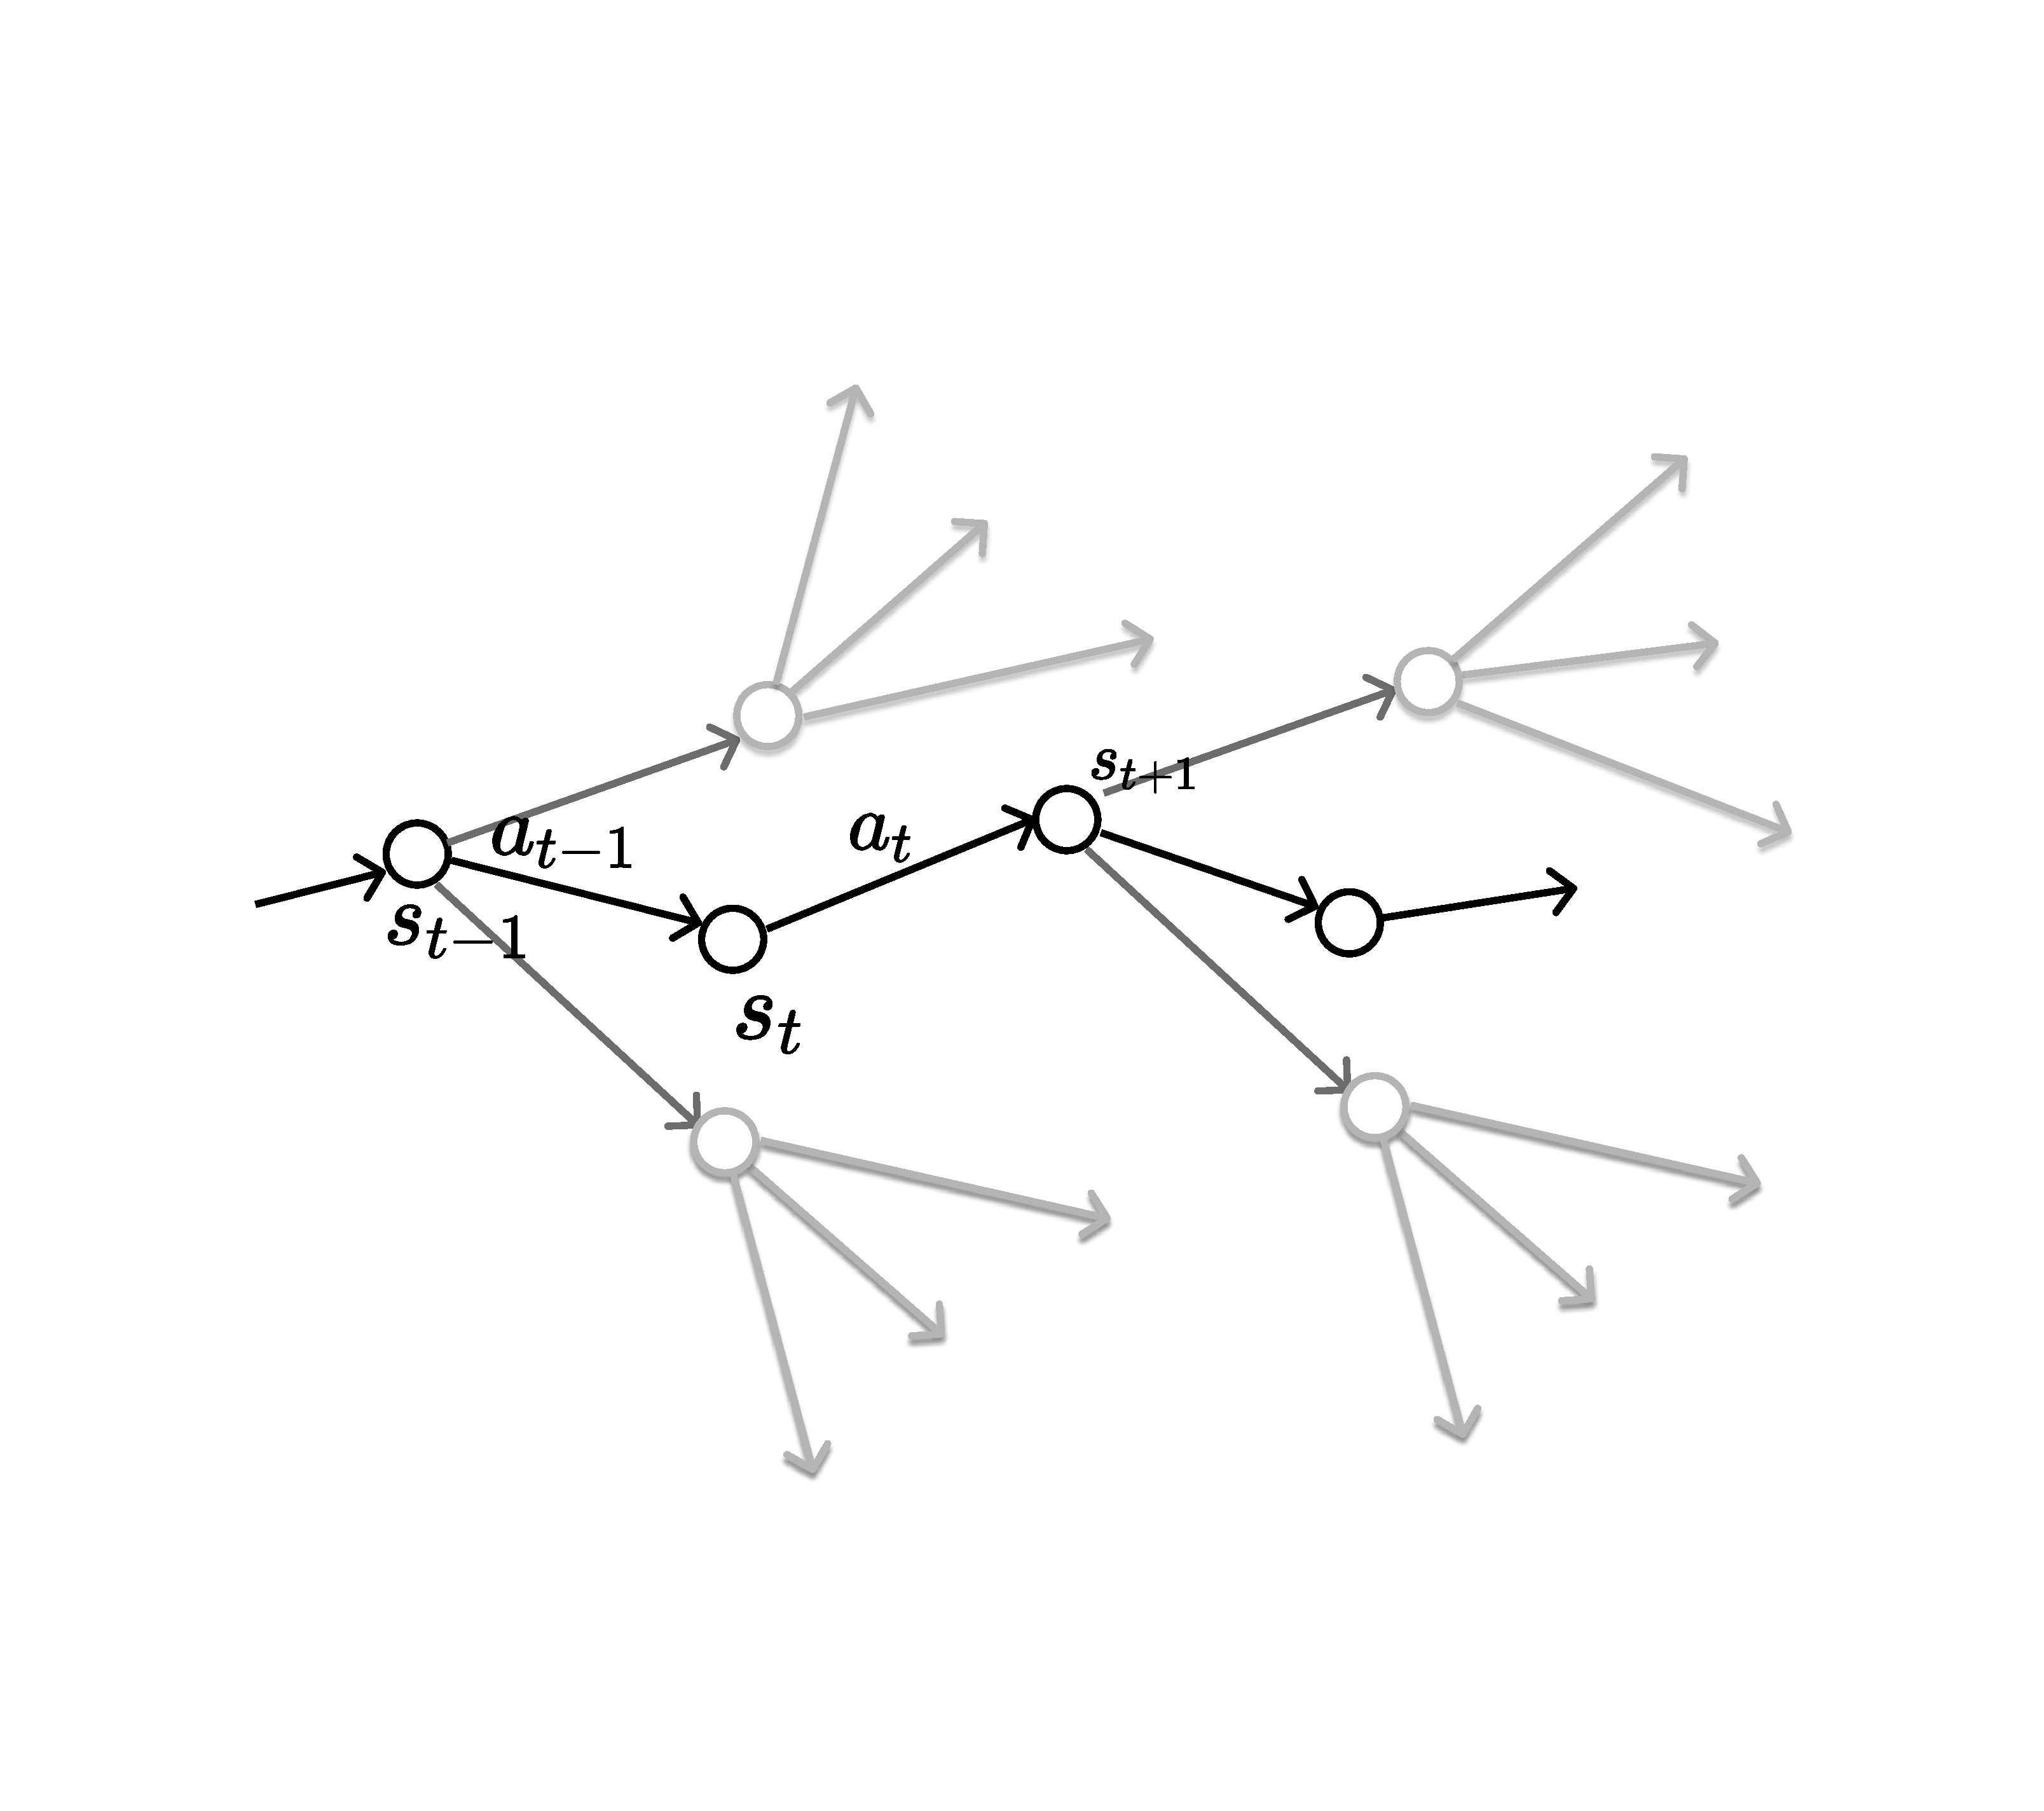
\includegraphics[width=0.45\textwidth]{figures/MDP.pdf}
    \caption{One can think of a Markov Decision Process as a tree of possible states $s_t, s_{t+1},...$ connected by branches associated with the transition probability function $P(s_{t+1}|s_t,a_t)$.}
\end{figure}

Given a POMDP, a discount factor $\gamma \in [0,1)$ and a policy function $\pi :\mathcal{S}\rightarrow\mathcal{A}$ we can compute the \textit{expected discounted reward} using the Bellman equation: 

\begin{align*}
    J{\pi_\theta} = \mathbb{E} \left[ \sum^\infty_{t=0} \gamma^t R(s_{t+1},s_t,\pi_\theta(o_t)) \right].
\end{align*}

The problem of reinforcement learning is formulated as the optimization of some parametrizable policy function $\pi$ (where the parameters are denoted $\theta$) over the POMDP process that ensures the the $J$ value is maximized in expectation across all states, i.e.:

\begin{align*}
    \pi^* = \text{argmax}_{\pi_\theta} \mathbb{E} \left[ \sum^\infty_{t=0} \gamma^t R(s_{t+1},s_t,\pi_\theta(o_t)) \right].
\end{align*}

\subsection{Policy Gradient Methods}

We will consider a \textit{policy gradient} reinforcement learning method, such an approach is the most natural for a continuous control task, these method work by directly updating a policy function rather than by computing an estimator of the discounted reward for all possible actions (which is what is done in Q-learning methods). Policy gradient RL methods use update rules of the form:

\begin{align*}
    \theta_{k+1} = \theta_k + \alpha \nabla_{\theta_k} J(\pi_{\theta_k}) \vert_{\theta_k}.
\end{align*}

Here the tricky part of the method resides in deriving an expression for the gradient $\nabla_{\theta_k} J(\pi_{\theta_k}) \vert_{\theta_k}$ of the expected reward $J$ with respect to the parameters $\theta$ of the policy $\pi$. These methods are often presented in MDP instead of POMDP form but they generalize well to POMDPs. The derivation of policy gradient is performed as follows:
\begin{align*}
    \nabla_{\theta_k} J(\pi_{\theta_k}) \vert_{\theta_k} 
    =  \nabla_{\theta_k} \int_\tau P(\tau|\theta)R(\tau)
    % && \text{}
    && \text{Expand expectation}\\
    =  \int_\tau \nabla_{\theta_k}  P(\tau|\theta)R(\tau)
    && \text{Use linearity}\\
    =  \int_\tau  P(\tau|\theta) \nabla_{\theta_k} \log P(\tau|\theta)R(\tau)
    && \text{Log trick} \\
    =  \underset{\tau \sim \pi_\theta}{\mathbb{E}} \left[\nabla_{\theta_k} \log P(\tau|\theta)R(\tau)\right]
    && \text{Take the expectations}\\
    =  \underset{\tau \sim \pi_\theta}{\mathbb{E}} \left[\nabla_{\theta_k} \sum_{t=0}^T \log \pi_\theta(a_t|s_t)R(\tau)\right]
    && \text{Expand over trajectories}
\end{align*}

Where $\tau$ denotes the set of all trajectories $s_0,a_0,s_1,a_1,...$ in the state space under policy $\pi_\theta$. In practice one can compute an estimate $\hat{g}$ of $\nabla_{\theta_k} J(\pi_{\theta_k})$ by sampling the MDP a sufficiently large number of time. Such an estimator is written out as follows: 

\begin{align*}
    \hat{g} = \frac{1}{|\mathcal{D}|} \sum_{\tau \in \mathcal{D}} \sum_{t=0}^{T} \nabla_\theta \log \pi_\theta (a_t|s_t) G_t,
\end{align*}
where $G_t$ is the expected discounted reward over the remaining steps in the episode.

\subsection{Advantage Actor Critic}

Policy gradient methods derived as we described above tend to lead to unstable learning. 
This is largely attributable to the fact that the gradient norms are subject to a high variance \cite{Konda00actor-criticalgorithms}.
The gradient in the variance of $\nabla_{\theta_k} J(\pi_{\theta_k})$ is proportional to the absolute value of the expected discounted reward over the trajectory $R(\tau)$, we can thus reduce the variance of our gradient estimator by subtracting a baseline to it's reward (this doesn't affect the gradients in expectation and thus the algorithm still converges to the same policy), the most common baseline used in that context is the \textit{on-policy value function $V_{\pi_\theta}(s)$}. 
This means a policy algorithm such as A2C we will have require two separate networks, an actor network (to implement a policy function) and a a critic network (to implement a value estimator) which both need to train simultaneously. To derive the formulation of advantage actor critic we first observe policy gradient implicitely makes use of $Q$ values.\\

\begin{align*}
    \hat{g} = \underset{\tau}{\mathbb{E}} \left[ \sum_{t=0}^{T} \nabla_\theta \log \pi_\theta (a_t|s_t) G_t \right] && \text{}\\
    = \underset{s_0,a_0,...}{\mathbb{E}} \bigg[ \big[ \sum_{t=0}^{T} \nabla_\theta \log \pi_\theta (a_t|s_t) G_t \big] && \text{Observe that:}\\
    + \underset{s_{t+1},r_{t+1},...,s_{T},r_{T}}{\mathbb{E}} [G_t] \bigg] && \mathbb{E} [G_t] = Q(s_t,a_t)\\
    = \underset{s_0,a_0,...}{\mathbb{E}} \bigg[ \sum_{t=0}^{T} \nabla_\theta \log \pi_\theta (a_t|s_t) Q(s_t,a_t) \bigg] && 
\end{align*}

Then we subtract the baseline $V$ as follows:
\begin{align*}
    \hat{g} = \frac{1}{|\mathcal{D}|} \sum_{\tau \in \mathcal{D}} \sum_{t=0}^{T} \nabla_\theta \log \pi_\theta (a_t|s_t) (G_t-V(s))\\
\end{align*}

Using the Bellman Optimality equation $Q(s_t,a_t) = \mathbb{E}[r_{t+1}] + \gamma V(s_{t+1})$ we have that can write out the advantage function as:
\begin{align*}
    A(s_{t+1},s_t,a_t) = Q(s_t,a_t) - V(s_t,a_t) \\
   \sim r_{t+1} + \gamma V(s_{t+1}) - V(s_t,a_t) 
\end{align*}

This approach leads us the the \textit{Advantage Actor Critic Method} (A2C) which computes it's gradients from an advantage function $A$ instead of a direct reward $R$:

\begin{align*}
    \hat{g} = \frac{1}{|\mathcal{D}|} \sum_{\tau \in \mathcal{D}} \sum_{t=0}^{T} \nabla_\theta \log \pi_\theta (a_t|s_t) A(s_{t+1},s_t,a_t)\\
    = \frac{1}{|\mathcal{D}|} \sum_{\tau \in \mathcal{D}} \sum_{t=0}^{T} \nabla_\theta \log \pi_\theta (a_t|s_t) (r_{t+1} + \gamma V(s_{t+1}) - V(s_t))
\end{align*}

In that framework we train two networks side by side, one of them is updated by the approximative gradient $\hat{g}$, and the other is updated by some loss function so that it converges to correct $V$ values.

\subsection{Proximal Policy Optimization}
\label{sec:ppo}


\begin{algorithm}
    \caption{PPO-Clip}
    \label{ppo-clip}
    Initialize neural networks $\pi_\theta$ and $V_\phi$ \\
    Set counter $t \leftarrow 0$, observe $s_0$ from the env \\
    \Repeat(){convergence}{
        \ForAll(){workers $k$}{
            \textbf{Take action} $a_t^{(k)} \leftarrow \pi_\theta(s_t^{(k)})$, \textbf{observe reward} $r_t^{(k)}$ and new state $s_{t+1}^{(k)}$\\
            Compute $R_t^{(k)} =  r_t^{(k)} + \gamma V_\phi(s_{t+1})$ and the advantage $A^{(k)}_t = R_t^{(k)} - V_\phi(s_{t})$\\
        }
        \textbf{Update the policy :} optimize the surrogate loss $\hat{L}^\text{CLIP}(\theta') = \sum_{k} \gamma^t \text{clip}(r_{\theta'}(s_t,a_t),1-\epsilon,1+\epsilon) A_\theta(s_t,a_t)$ with gradient descent for $M$ epochs\\
        \textbf{Update the advantage estimator :} $\phi$ by the gradient of $\sum_K (R_t^{(k)} - V_\phi(s_t^(k)))^2$
    }
\end{algorithm}


Starting from A2C one can get further improvements in the stability of the convergence by constraining gradient descent to a small region in parameter space for each mini-batch. Algorithms making use of this idea (Trust Region Policy Optimization and Proxy Policy Optimization \cite{Schulman2017ProximalPO}) are giving state of the art results for continuous control tasks. A really nice walkthrough of this derivation can be found in Johanni Brea's lecture notes \cite{Brea} for the course Artificial Neural Networks at EPFL. \\

A rough intuition of why these methods work can be gathered from writing out the expected policy improvements $J(\theta') - J(\Theta)$ of A2C. 
{\tiny
\begin{align*}
    J(\theta') - J(\theta) = J(\theta') - \underset{s_0 \sim p(s_0)}{\mathbb{E}} [V_\theta(s_0)] 
    && \parbox{8em}{By def. of $J(\theta)$} \\
    = J(\theta') - \underset{s_t,a_t \sim \theta'}{\mathbb{E}} [V_\theta(s_0)] 
    && \parbox{8em}{Take the expectation over all state action pairs (for policy $\pi(\theta')$)} \\
    = J(\theta')  
    - \underset{s_t,a_t \sim \theta'}{\mathbb{E}} \left[ \underbrace{\sum_{t=0}^\infty \gamma^t V_\theta(s_t) - \sum_{t=1}^\infty \gamma^t V_\theta(s_t)}_{\sum_{t=0}^\infty \gamma^t [V_\theta(s_t) - \gamma V_\theta(s_t) ]}\right]
    && \parbox{8em}{Write out the expectation as a collapsing sum}\\
    =  \underset{s_t,a_t \sim \theta'}{\mathbb{E}} \left[ \sum_{t=0}^\infty \gamma^t \underbrace{[r^{a}_{s_t \rightarrow s_{t+1}} - \gamma V_\theta(s_{t+1}) - V_\theta(s_{t}) ]}_{A_\theta(s_t,a_t)}  \right]
    && \parbox{8em}{Plugging in the definiton of $J(\theta')$}\\
    =  \underset{s_t,a_t \sim \theta'}{\mathbb{E}} \left[ \sum_{t=0}^\infty \gamma^t A_\theta(s_t,a_t)  \right] && \parbox{8em}{By definiton of the advantage function}\\
    = \underset{s_t,a_t \sim \theta}{\mathbb{E}} \left[ \sum_{t=0}^\infty \gamma^t \frac{\pi_{\theta'}(s_t,a_t)}{\pi_{\theta}(s_t,a_t)} A_\theta(s_t,a_t)  \right]
    && \parbox{8em}{Taking expectation over $\pi(\theta)$ instead of $\pi(\theta')$)}.\\
\end{align*}}


We observe that the expected improvement is maximized in expectation when the  term $\gamma^t \frac{\pi_{\theta'}(s_t,a_t)}{\pi_{\theta}(s_t,a_t)} A_\theta(s_t,a_t)$ is maximized. Assuming that the updated policy is close to the previous parametrization (i.e. $\frac{\pi_{\theta'}(s_t,a_t)}{\pi_{\theta}(s_t,a_t)} \approx 1$). We can directly optimize (maximize) an estimator of the improvement that we call $\hat{L}(\theta')$:

\begin{align*}
    \hat{L}(\theta') = \sum^\infty_{t=0} \gamma^t \overbrace{ \frac{\pi_{\theta'}(s_t,a_t)}{\pi_{\theta}(s_t,a_t)}}^{=r_{\theta'}(s_t,a_t) \approx 1} A_\theta(s_t,a_t).
\end{align*}


There are several approaches to keep the updated policy "close" to the previous installment ($r_{\theta'}(s_t,a_t) \approx 1$), one of the is theM compute an estimator of the KL divergence between both policies (which is what is done in TRPO) another is simply clip the loss at some maximum according to the following clipping function: 

\begin{align*}
    \text{clip}(x,\mu,\nu) =  
    \begin{cases}
        \nu & \text{if}~x<\nu \\
        x & \text{if}~\nu<x<\mu \\
        \mu & \text{if}~\mu<x 
    \end{cases}.
\end{align*}

We called the clipped loss function the "\textit{surrogate loss}". This gives rise to the \textit{PPO-Clip} algorithm for which we give a pseudocode implementation in algorithm \ref{ppo-clip}.  \\

\begin{algorithm}
    \caption{Batched PPO-Clip}
    \label{batched-ppo-clip}
    Initialize neural networks $\pi_\theta$ and $V_\phi$ \\
    Set counter $t \leftarrow 0$, observe $s_0$ from the env \\
    \Repeat(){convergence}{
        Initialize a trajectory batch $\tau \leftarrow (\tau^{(1)},\tau^{(2)},...,\tau^{(k)})$\\
        \For{$t\in[0,\text{episode lenght}]$}{
            \ForAll(){workers $k$}{
                \textbf{Take action} $a_t^{(k)} \leftarrow \pi_\theta(s_t^{(k)})$, \textbf{observe reward} $r_t^{(k)}$ and new state $s_{t+1}^{(k)}$\\
                Compute $R_t^{(k)} =  r_t^{(k)} + \gamma V_\phi(s_{t+1})$ and the advantage $A^{(k)}_t = R_t^{(k)} - V_\phi(s_{t})$\\
                Append $s_t^{(k)},a_t^{(k)},s_{t+1}^{(k)},x_t^{(k)},R_t^{(k)},A^{(k)}_t$ to the trajectory $\tau^{(t)}$ associated with the worker
            }
        }
        
        \While(){trajectory batch $\tau$ is not empty}{
            sample mini-batch from $\tau$ (and remove sampled elements) \\
            \textbf{Update the policy :} optimize the surrogate loss over sampled mini-batch $\hat{L}^\text{CLIP}(\theta') = \sum_{k} \gamma^t \text{clip}(r_{\theta'}(s_t,a_t),1-\epsilon,1+\epsilon) A_\theta(s_t,a_t)$ with gradient descent for $M$ epochs\\
            \textbf{Update the advantage estimator :} $\phi$ by the gradient of $\sum_K (R_t^{(k)} - V_\phi(s_t^(k)))^2$ over sampled mini-batch
        }
    }
\end{algorithm}

This reference implementation assumes that the policy is updated as the policy goes through environment steps. In practice this causes trouble when implementing the algorithm as it forces the batch size $k$ to be directly fixed by the number of parallel workers. An alternative approach consists in sampling the environment for several steps (we call this sequence of steps an "\textit{episode}") and then to reconstitute batches after the fact for training. This is what we will implement for our experiments. Algorithm \ref{batched-ppo-clip} gives pseudocode for such an implementation.




\subsection{An architecture for training CTNNs using PPO}

Dealing with the continuous time nature of the CTNN cells doesn't cause much trouble when implementing a reinforcement learning algorithm as it mostly just changes the back-propagation algorithm but not the loss or the variables that need to be stored in the process. On the other hand the fact that our CTNN cells are recurrent (have an inner state) changes the process as we somehow need to implement the \textit{unrolling} of the inner states. \\

The way we do it is by saving the inner states $x_i^{(t)}$ of each neuron at each time step in every trace and then to consider them to be observations when training the policy, this allows for a minimal amount of changes to the PPO architecture at the cost of a relatively high memory use.